\section{Hierarchical VMP system: Snooze}

We now present Snooze~\cite{feller:ccgrid12} as a representant of the
class of hierarchical VMP systems.  We first present its architecture
summarizing its main characteristics from its original
presentation~\cite{feller:ccgrid12} and additional information
stemming from personal communications of the Snooze developers and its
implementation~\cite{snoozeweb,snoozedev14}. We then present detailed
analyses of several of its major characteristics, notably relating to its
fault tolerance.

\subsection{System overview}

\subsubsection{Architecture}

~ \MS{From Euro-Par: to be rewritten}

Snooze~\cite{snoozeweb,feller:ccgrid12} harnesses a hierarchical
architecture in order to support load balancing and fault tolerance,
cf.\ Fig.~\ref{fig:snoozearch}.
At the top, %of the hierarchy,
 a \emph{group leader (GL)} centralizes information about the whole
cluster using summary data about \emph{group managers (GMs)} that
constitute the intermediate layer of the hierarchy. GMs manage a
number of \emph{local controllers (LCs)} that, in turn, manage the VMs
assigned to nodes.
% The GL and the GMs are deployed on service nodes while the LCs are
% executed on hosting node.

\begin{figure}\centering
  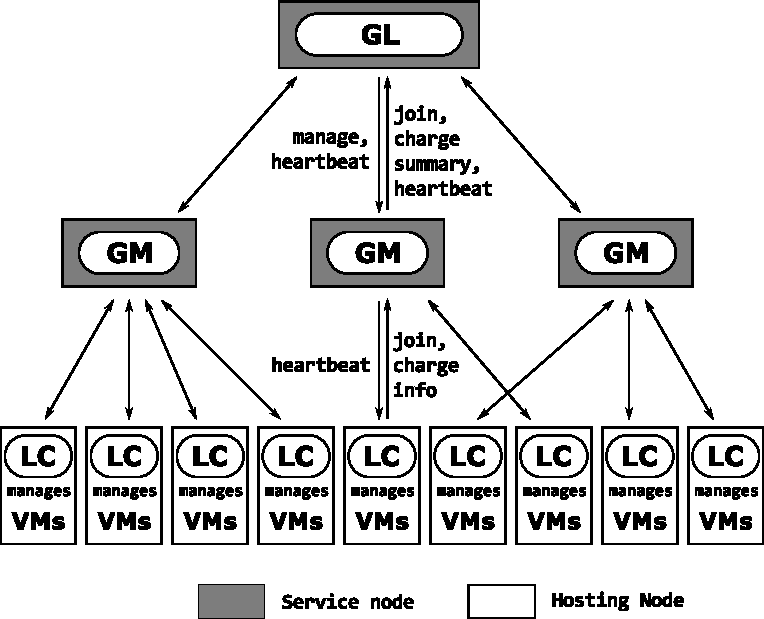
\includegraphics[width=.9\linewidth]{figures/snooze/snoozearch.pdf}
  \caption{Snooze Architecture}
  \label{fig:snoozearch}
\end{figure}
During execution, higher-level components periodically send heartbeats
to lower-level ones; monitoring information, \eg about the system
load, is also sent periodically in the opposite direction. In order to
propagate information, Snooze relies on hardware support for multicast
communication.
% Finally, entry points allow clients to contact the GL, \eg to submit
% new VMs for integration into the system.

The implementation in \vmps of the core architectural abstractions of
Snooze % (\ie VM monitoring and manipulations)
leverages the \texttt{XHOST}, \texttt{XVM} and
\texttt{SimulatorManager} while other mechanisms have been implemented
using Simgrid's primitives and standard Java mechanisms.

For instance, communication between Snooze actors is implemented based
on Simgrid's primitives for, mainly asynchronous, event handling.  The
multicast capability that is used, \eg to relay heartbeats, is
implemented as a dedicated service that manages a state to relay
heartbeat events in a concurrent manner to all receivers.

Finally, our Snooze simulation uses, as its original counterpart, a
multi-threaded implementation (\ie based on multiple \sg processes) in
order to optimize reactivity even for large groups of LCs (or GMs)
that have to be managed by one GM (or GL).

\subsubsection{Algorithms}
\label{sec:snoozeAlgs}

~ \MS{New}

Apart from the handling of faults (described below), two types of
algorithms are of major importance for the administration of the
Snooze architecture: the algorithms that enable components to
dynamically enter the system and the algorithms that propagate info
between the components.

A GL is created, if it does not exist, by promotion of a GM that is
selected according to some leader election algorithm. When a GM joins
a cluster, it starts listening on a predefined channel for the
heartbeat of the GL and registers once it has received the
heartbeat. New LCs first also wait for the GL heartbeat, contact the
GL then in order to obtain a GM assignment, and finally register at
the GM assigned to them.

Two kinds of (load) information are passed within the system: the
periodic heartbeat message sent by the GL and the GMs; second,
periodic load information sent from LCs to their respective GMs and
summary load info sent by the GMs to the GL.

\subsubsection{Fault tolerance}

~ \MS{New}

GLs, GMs and LCs may fail during the system execution. System
components identify that a node on the corresponding higher-level node
has failed (the GL in case of a GM, a GM in the case of an LC) in an
asynchronous fashion through the lack of heartbeat messages.

In the case of a GL failure, one of the GMs becomes the new GL, stops
its GM activities and prevents the LCs it manages so that they can
start rejoining the system. If a GM fails, the GL and the LCs it has
managed will become aware of it based on the lack of heartbeats,
update its data structures and, for the LCs, rejoin the system. If an
LC fails, its GM will finally learn of it due to the missing heartbeat
and charge information of the LC. The GM will then remove the LC from
its data structures.

\subsection{Analysis}


\subsubsection{Varying group sizes}


\begin{figure*}[t]

\subcapcentertrue
%\subfigure[Total Violation Times]{
\subfigure{
  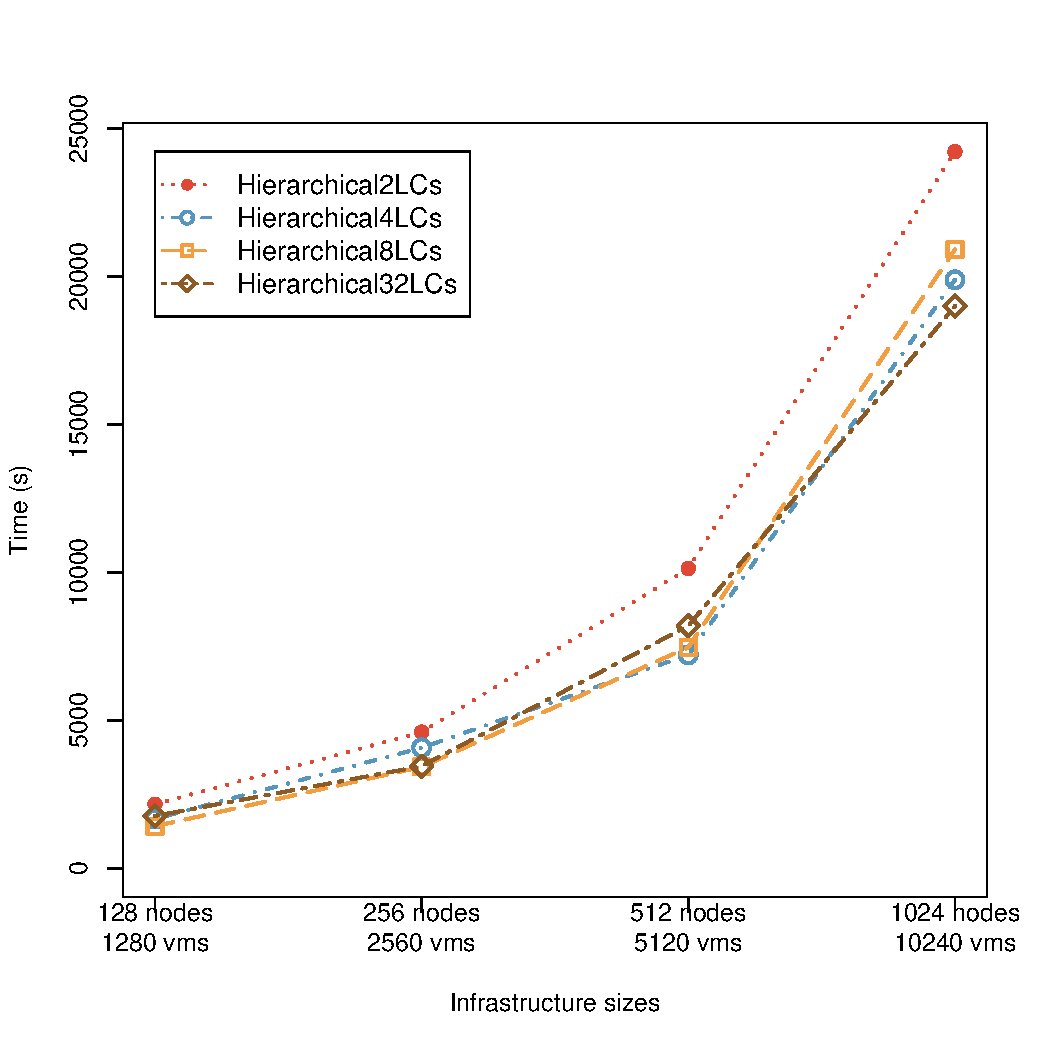
\includegraphics[width=.38\textwidth]{figures/snooze/groupSizes-violationTime.pdf}
  \label{fig:groupSizesViolationTime}}
% \begin{minipage}{.60\textwidth}\centering

% %\subfigure[No.\ of Failed Reconfigurations]{
% \subfigure{
%     {\tiny \begin{tabular}[b]{|r@{\:}||@{\:}r@{\:}|@{\:}r@{\:}|@{\:}r@{\:}|@{\:}r@{\:}|}
%       \thickhline
%       \textbf{Infra.\ Size~~}
%         & \multicolumn{ 4 }{c@{\:}|}{No.\ of \textbf{failed reconfigurations}}
%           \Tstrut \\
%          \hfill &  ~2 LCs~ & ~4 LCs~ & ~8 LCs~ &  ~32 LCs~  \Bstrut \\
%       \thickhline

%         128~~~~~~~ &  19~ & 0~ & 0~ & 0~ \\
%         256~~~~~~~ &  29~ & 0~ & 0~ & 0~ \\
%         512~~~~~~~ &  83~ & 1~ & 0~ & 0~ \\
%        1024~~~~~~~ & 173~ & 7~ & 0~ &  0
%       \Rstrut  \\ \hline
%       \thickhline
%   \end{tabular} }
%   \label{fig:groupSizesReconfigFail}
%   }

% %\subfigure[Means $\pm$ Std deviations of computation durations.]{
% \subfigure{
%     {\tiny \begin{tabular}[b]{|r@{\:}||@{\:}c@{\:}|@{\:}c@{\:}|@{\:}c@{\:}|@{\:}c@{\:}|}
%       \thickhline
%       \textbf{Infra.\ Size~~}
%         & \multicolumn{ 4 }{c@{\:}|}{Duration of the
%             \textbf{computations $(\mu \pm \sigma)$}}
%           \Tstrut \\
%          \hfill &  ~2 LCs~ & ~4 LCs~ & ~8 LCs~ & 32 LCs  \Bstrut \\
%       \thickhline

%         128~~~~~~~ &   0.16 $\pm$   1.23 &   0.34 $\pm$   1.81 &   0.58 $\pm$   2.40 &   2.53 $\pm$   4.62  \\
%         256~~~~~~~ &   0.18 $\pm$   1.31 &   0.42 $\pm$   1.99 &   0.66 $\pm$   2.50 &   2.65 $\pm$   4.69  \\
%         512~~~~~~~ &   0.15 $\pm$   1.20 &   0.33 $\pm$   1.78 &   0.67 $\pm$   2.54 &   2.83 $\pm$   4.98  \\
%        1024~~~~~~~ &   0.19 $\pm$   1.37 &   0.42 $\pm$   2.02 &   0.89 $\pm$   2.90 &   ~2.69 $\pm$   4.91

%       \Rstrut  \\ \hline
%       \thickhline
%   \end{tabular} }
%   \label{fig:groupSizesComputationTime}
%   }
% \end{minipage}

\caption{Hierarchical placement: influence of varying group sizes}
\label{fig:snoozeGroupSizes}

\end{figure*}

~ \MS{From Euro-Par: to be extended and rewritten; tables don't compile}

\vmps facilitates the in-depth analysis of variants of placement
algorithms. We have, for example, analyzed, as a first study of its
kind, how the Snooze-based placement depends on the no.\ of LCs
assigned to a GM. Fig.~\ref{fig:snoozeGroupSizes} presents the
simulated values obtained for scenarios with 2,~4,~8 and 32~LCs per GM
for four infrastructure sizes. The overall performance (\ie cumulated
violation time) shows that 2~LCs per GM result in significantly higher
violation times.
% All other
%group sizes yield violation times that are relatively close, which
%indicates that a small group size does not help much in
%resolving violations faster.
The relatively bad performance of the smallest group size can be
explained in terms of the number of failures of the reconfiguration
process, that is, overloading situations that are discovered but
cannot be resolved
% because the GM managing the overloaded VM(s) did not dispose of
% enough
due to a lack of resources (see tables on the right).  Groups of 2~LCs
per GM are clearly insufficient at our global load level (85\%).
Failed reconfigurations are, however, already very rare in the case of
4~LCs per GM and do not occur at all for 8~and 32~LCs per GM. This is
understandable because
% the load is statistically evenly distributed among the LCs and
the load profile we evaluated rarely results in many LCs of a GM to be
overloaded at once. Violations can therefore be resolved even in the
case of a smaller number of LCs available for load distribution.
Conversely, we can see that the duration of the computation phases
decreases strongly along with the group size. It reaches a value close
to the computation times of DVMS for a group size of 4-LCs per
GM.% see Fig.~\ref{fig:groupSizesComputationTime}.
We thus cannot minimize computation times and violation times by
reducing the number of LCs because larger group sizes are necessary to
resolve overload situations if the VM load gets higher.  In contrast,
DVMS resolves this trade-off by means of its automatic and dynamic
choice of the partition size necessary to handle an overload
situation.  Once again, this information is valuable as it will help
researchers to design new algorithms favoring the automatic discovery
of the optimal subset of nodes capable to solve violations for given
load profiles.


\subsubsection{Fault tolerance} 

\MS{New. To be extended}

\begin{figure}\centering
  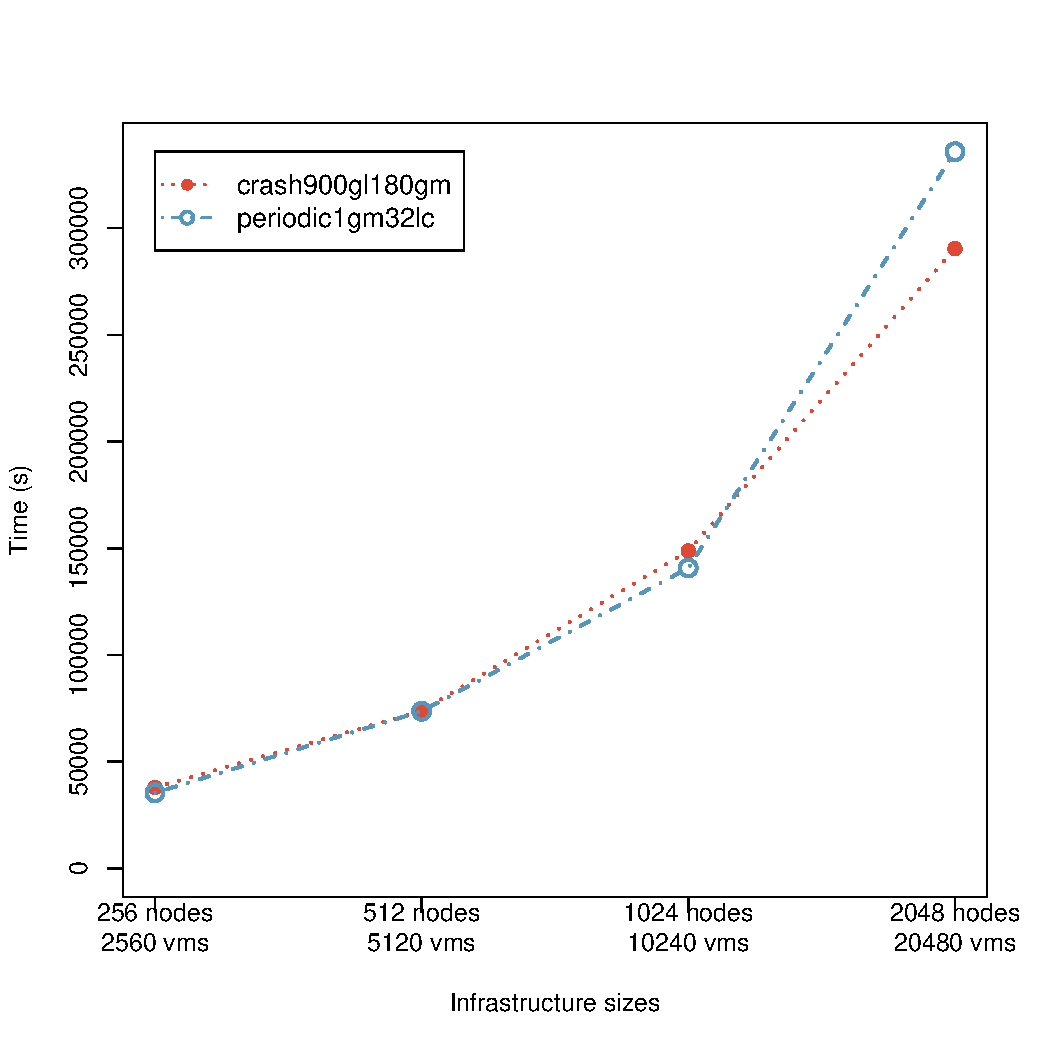
\includegraphics[width=.45\linewidth]{figures/snooze/crashAbs-reconfiguration.pdf}
  \quad
  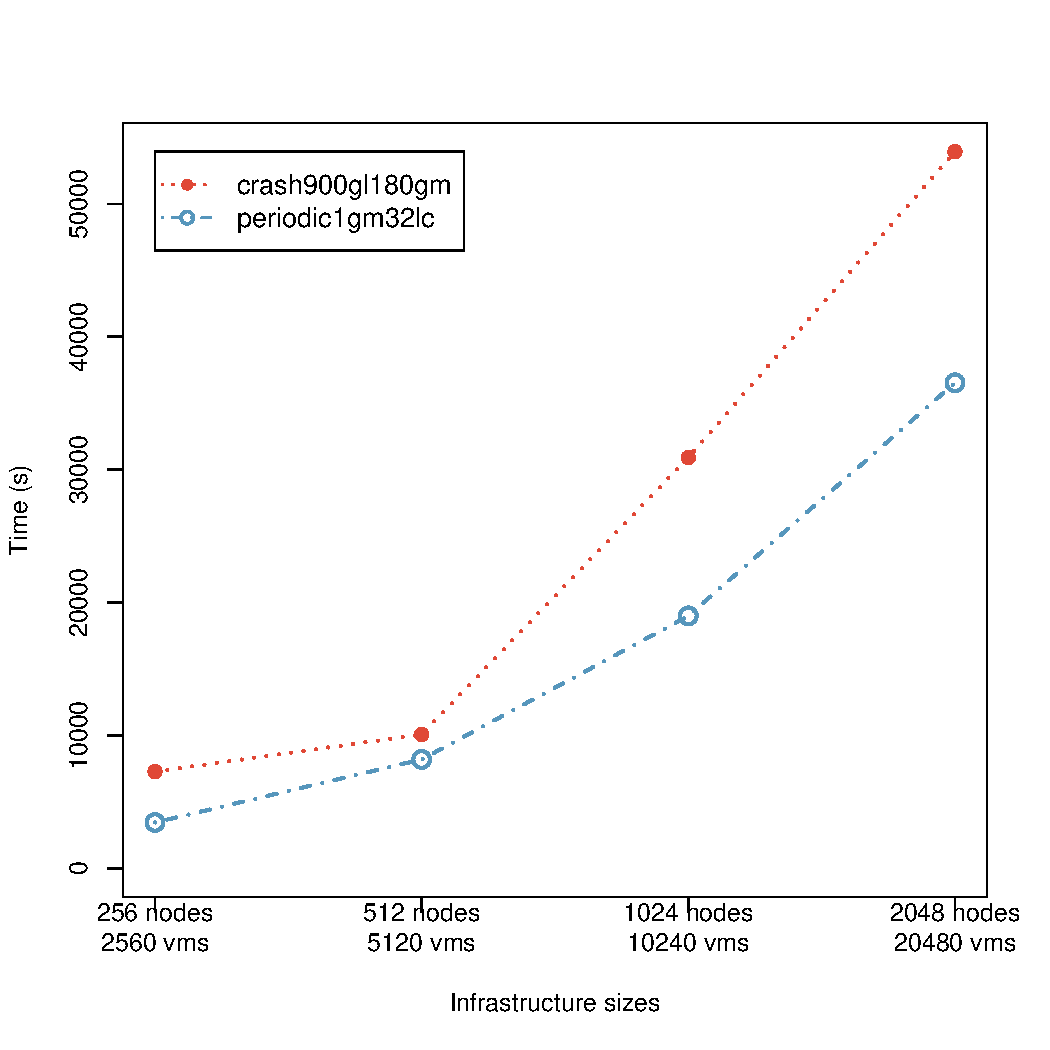
\includegraphics[width=.45\linewidth]{figures/snooze/crashAbs-violation.pdf}
  \caption{Behavior in the presence of faults}
  \label{fig:snoozeFaults}
\end{figure}

Figure~\ref{fig:snoozeFaults} shows the total reconfiguration times
(left) and violation times (right) in the presence of faults over
1800s for infrastructure sizes of 256, 512, 1024 and 2048 LCs. The
simulations have been calibrated so that 8~GM~faults and 1~GL~fault
are generated over the total period, a rather small fault rate.

These results clearly show that while the total reconfiguration times
is not much affected by the faults (because the total number of
available LCs per GM remains roughly constant), the violation time is
strongly affected (because the faults disturb on-going and future
resolution actions triggered by violations).
\MS{Are the above reasons correct?}

\MS{Analyze other fault configurations.}

\subsection{Algorithm variants}

~ \MS{New: from HPDC draft}


We now present three non-trivial variants that we have implemented and
explored: periodic vs.\ reactive scheduling, a variant of the
assignment algorithm of LCs to GMs, and a variant of the algorithms of
how GMs and LCs join the system.  \MS{How and where do we provide the
  scheduling parameters for the evals.?}

\subsubsection{Periodic vs.\ reactive scheduling}

Snooze~\cite{feller:ccgrid12} schedules VMs in a periodic fashion:
after a fixed time period a GM calls the scheduler in order to resolve
resource conflicts among the LCs it manages. The information whether a
resource conflict has to be handled is taken based on the summary
information that is periodically sent by the LCs to the GM.

We have implemented using \vmps an alternative, reactive, strategy to
scheduling: as soon as resource conflicts occur, LCs avert their GMs
ofthem; the GMs then immediately initiate scheduling. Implementing
this reactive scheme can be done using our framework in two
manners. First, by implementing additional asynchronous transmissions
of the necessary state updates as a real implementation would
proceed. Second, in a much more lightweight manner through direct
accesses by the GMs to the states of their respective LCs. In order to
ensure that this leightweight implementation mimics a real
implementation closely, delays induced by communication in the
``real'' implementation are accounted for (congestion issues are not
relevant in this case because a resource conflict blocks the GM and
its LCs anyway). We have implemented this lightweight variant of
reactive scheduling including explicit modeling of communication
delays. Using the abstractions provided by \vmps, in particular
harnessing its extended notion of hosts that represent the VMs managed
by the LCs of a VM, reactive scheduling has been implemented by adding
4~lines of code.

\begin{table*}[ht]
\begin{center}
\begin{tabular}{|P{30mm}||c|c|c|c||c|c|c|c|}
    \thickhline
    \textbf{Algorithm}
      & \multicolumn{4}{c||}{\textbf{No.\ migrations}}
      & \multicolumn{4}{c|}{\textbf{Total violation time (s)}}
      \Tstrut \\
    \textbf{\#LCs/\#GMs}  & 64/6 & 128/12 & 256/25 & 512/51 &  64/6 & 128/12 & 256/25 & 512/51 \Bstrut \\ 
    \thickhline
      Reactive      & 30 & 89 & 179 & 338 & 267 & 764 & 1638 & 3088 \\
      Periodic 120s & 9 & 24 & 69 & 142 & 814 & 2548 & 6238 & 16038
    \Rstrut \\ \hline
    \thickhline
\end{tabular}
\end{center}
    \caption{Reconfiguration nos. and violation times for reactive and
    periodic scheduling}
\label{tbl:reactiveRes}
\end{table*}

We have shown the usefulness of our framework by exploring some
properties of reactive scheduling compared to periodic scheduling. To
this end we have simulated reactive scheduling and a periodic
algorithm that reconfigures all LCs every 2 mins for configurations
ranging from 64 to 512 LCs. These simulations have yielded, among
others, the results shown in Tbl.~\ref{tbl:reactiveRes}. The results
clearly show that while a reactive strategy entails a much higher
number of migrations (because the periodic one misses many overload
situations), reactive scheduling results in a significantly lower
total migration time.


\subsubsection{Assignment of LCs to GMs}

LCs are assigned to GMs by the GL as part of the LC join protocol. In
Snooze's native implementation LCs are assigned in a round-robin
fashion to the known GMs. If GMs join (and leave) the system at the
same time as LCs, a round-robin (RR) strategy at join time, however,
does not ensure an even distribution. This may happen, for instance at
startup time of the system, when new GMs and LCs enter the system, or
in case of failures, which trigger GM and LC joins. In order to
evaluate the corresponding imbalance and its consequences we have
implemented the LC assignment protocol in a modular fashion and
applied it to different highly-dynamic settings in which GMs and LCs
enter the system at the same time. Furthermore, we have implemented a
best-fit (BF) strategy that assigns LCs to the GMs with minimal load
or, if several GMs with minimal load exist, to the GMs with the
smallest number of assigned LCs.


% \subsubsection{LC assignment in Snooze-like placement alg.}
% \label{sec:snoozeVariantsEval}

% \begin{figure}[ht]
% \begin{center}
%     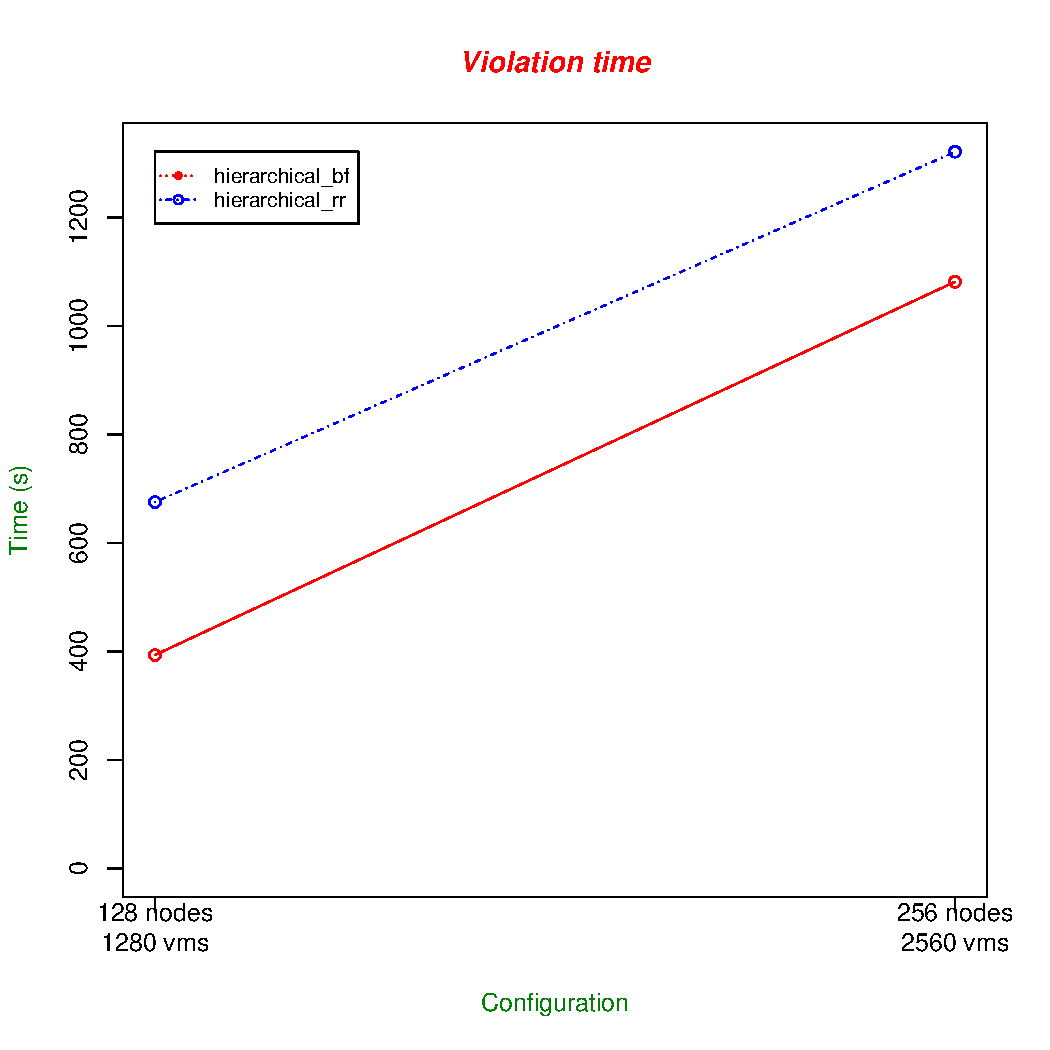
\includegraphics[width=.95\linewidth]{figures/violationTime-snooze-RR-BF.pdf}
%     \caption{Cumulated violation time for BF (lower line) and RR
%       (upper line) variants}
% \end{center}
% \label{fig:snoozeBFRRViolation}
% \end{figure}

\begin{table*}[ht]
\begin{center}
%    \begin{tabular}{|c!{\vrule width 3pt}c|c|c!{\vrule width 2pt}c|c|c!{\vrule width 3pt}c|c!{\vrule width 2pt}c|c|}
    \begin{tabular}{|P{30mm}|||c|c||c|c|||M{30mm}|M{30mm}|}
        \thickhline
        \multirow{3}*{\textbf{Strategy}}
          & \multicolumn{4}{c|||}{\textbf{\#LCs/\#GMs}}
          & \multicolumn{2}{c|}{\textbf{Total violation time (s)}}
          \Tstrut \\
          & \multicolumn{2}{c||}{128 LCs, 12 GMs}
            & \multicolumn{2}{c|||}{256 LCs, 25 GMs}
          & \multirow{2}*{128 LCs, 12 GMs} & \multirow{2}*{256 LCs, 25 GMs} 
          \Bstrut \\ 
          & range & stdev & range & stdev & &  \Bstrut \\
        \thickhline
        Best-Fit & 0--30 & 10.53 & 0--18 & 6.62  & 395 & 1005 \Rstrut \\
        Round-Robin & 0--49 & 15.7  & 0--35 & 12.22 & 630 & 1265
        \Rstrut \\ \hline
        \thickhline
    \end{tabular}
\end{center}
    \caption{LCs to GM assignment and cumulated violation times for RR
      and BF strategies}
    \label{tbl:assignmentResults}
\end{table*}


We have evaluated the two LC assignment strategies using \vmps on
configurations of~128 and~256 nodes. In order to clearly expose the
corresponding differences this evaluation has been performed by
``stressing'' the two strategies by simultaneously
starting all LCs (128/256) and all GMs (12/25) and then simulating the
resulting configuration over a one hour period.  These experiments
have yielded the following results, cf.\ Table~\ref{tbl:assignmentResults}:
\begin{itemize}
  \item BF yields more homogeneous assignments of LCs to GMs: the
    ranges of the numbers of LCs assigned to a GM and their standard
    deviations are significantly smaller.\footnote{Here, some GMs may
      be assigned 0 LCs if some GMs join the system after all LCs have
      been assigned.}
  \item The cumulated time spent resolving violations is, for both
    configurations, significantly smaller for BF than for RR.
\end{itemize}
From these results, we can clearly infer that BF is significantly
better than RR for the two tested kinds of configuration. Furthermore,
we conjecture that BF should perform at least as good as RR for all
configurations (the proof is left to future work).
% \MS[JP]{I need the exact figures for the violation times
%   in Tbl.~\ref{tbl:assignmenResults}}

\subsubsection{Variants of the join algorithms}

The join algorithms, see Sec.~\ref{sec:snoozeAlgs}, are crucial to
Snooze for two main reasons: (i) they have to be efficient because
they can easily form a bottleneck if large numbers of LCs (GMs) have
to be registered at a GM (LC); (ii) they are multi-phase protocols
whose correctness especially in the presence of faults is difficult to
ensure.

In order to investigate the corresponding trade-offs, we have used our
framework to implement join algorithms that may be interrupted at any
time, repeat the the on-going phase a number of times before
reinitiating, if necessary, the entire protocol. Furthermore, the join
protocol is parameterized, \eg, in the number of threads used to
handle registration requests.

Finally, our framework has enabled us to test another aspect of
Snooze's join algorithm as presented by
Feller~\etal.~\cite{feller:ccgrid12}, a strategy we call the GM rejoin
strategy (GRJ): all GMs and the LCs assigned to them should rejoin if
a new GM enters the system. While GRJ supports a form of load
balancing (because all LCs are reassigned to the new set of GMs), our
simulation has shown that this strategy significantly increases the
time necessary for registering GMs and LCs compared to a simpler
strategy that does not modify existing GMs in case a new GM enters the
system. This handicap is particularly pronounced if joins of GMs may
be interrupted due to faults. Concretely, experiments involving 20 GMs
and 200 LCs have shown that this strategy often multiplies the time
necessary to join all 220 components by 10 or more compared to the
simple join strategy. While the qualitative result that the more
complex strategy presented in the paper results in a more
time-consuming join process is not very surprising, the extent of the
resulting degradation was surprising.

